\section{Gronwall估计}
\label{sec:odesens-gronwall}

没有解的公式，怎样比较两条解曲线？回到积分形式。解是右端的累积，两条解的差也就是右端之差的累积，而右端之差又可以由解的差控制。这样得到一个把未知量放在两边的不等式，Gronwall不等式负责把它解开。

\paragraph{两条积分方程相减}
设$\bm{x}$和$\bm{y}$在$[t_0,T]$上绝对连续，分别满足
\[
 \dot{\bm{x}}=\bm{f}(t,\bm{x}),\qquad
 \dot{\bm{y}}=\bm{f}(t,\bm{y})+\bm{r}(t),
\]
初值为$\bm{x}(t_0)=\bm{x}_0$，$\bm{y}(t_0)=\bm{y}_0$，方程几乎处处成立。这里$\bm{r}(t)$是第二条曲线相对于方程的\term{残差}（residual），表示每一时刻额外多出来的变化率。写成积分形式，
\[
 \begin{aligned}
 \bm{x}(t)&=\bm{x}_0+\int_{t_0}^{t}\bm{f}(s,\bm{x}(s))\,\mathrm{d}s,\\
 \bm{y}(t)&=\bm{y}_0+\int_{t_0}^{t}\bigl[\bm{f}(s,\bm{y}(s))+\bm{r}(s)\bigr]\,\mathrm{d}s.
 \end{aligned}
\]
记$\bm{e}(t)=\bm{y}(t)-\bm{x}(t)$，$\bm{e}_0=\bm{y}_0-\bm{x}_0$。两式相减，得到
\[
 \bm{e}(t)=\bm{e}_0+\int_{t_0}^{t}\bigl[\bm{f}(s,\bm{y}(s))-\bm{f}(s,\bm{x}(s))\bigr]\,\mathrm{d}s+\int_{t_0}^{t}\bm{r}(s)\,\mathrm{d}s.
\]

现在设右端关于状态满足Lipschitz条件，在时刻$s$的常数为$L(s)$，也就是
\[
 \lVert\bm{f}(s,\bm{y}(s))-\bm{f}(s,\bm{x}(s))\rVert_2\leq L(s)\lVert\bm{e}(s)\rVert_2.
\]
取范数并用三角不等式，$u(t)=\lVert\bm{e}(t)\rVert_2$满足
\begin{equation}
 u(t)\leq\lVert\bm{e}_0\rVert_2+\int_{t_0}^{t}\bigl[L(s)u(s)+\lVert\bm{r}(s)\rVert_2\bigr]\,\mathrm{d}s.
 \label{eq:odesens-error-inequality}
\end{equation}
式~\eqref{eq:odesens-error-inequality}两边都有$u$，并没有给出$u$的上界：要知道今天的误差，得先知道过去的误差。

\paragraph{复利的图景}
把$u$看成账户余额，$L(s)$是时刻$s$的利率，$\lVert\bm{r}(s)\rVert_2$是时刻$s$的存款速度，$\lVert\bm{e}_0\rVert_2$是本金。一小段时间$h$内，余额至多变成
\[
 u(s+h)\lesssim\bigl(1+L(s)h\bigr)u(s)+\lVert\bm{r}(s)\rVert_2h.
\]
这正是复利的递推。复利的结果可以直接写出：本金从$t_0$起计息，到$t$时乘以$\exp\int_{t_0}^{t}L$；时刻$s$存入的一小笔钱只从$s$起计息，到$t$时乘以$\exp\int_{s}^{t}L$。

图~\ref{fig:odesens-gronwall-deposits}画出了这两种钱的去向。类比也有限度：账户的利率真实发生，而式~\eqref{eq:odesens-error-inequality}只说误差“至多”按这个利率增长，真实的误差可能增长得慢，甚至缩小。Gronwall不等式给出的因此只是上界。

\begin{BookInlineFigure}
  \centering
  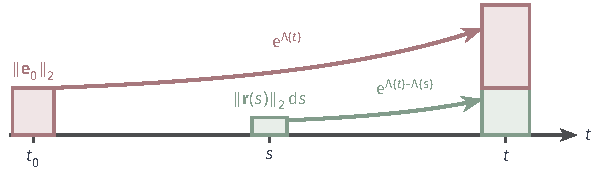
\includegraphics[width=101.9mm]{figures/06-differential-equations/01-ordinary-differential-equations/tikz/odesens-gronwall-deposits/figure.pdf}
  \caption{误差的复利账本示意。红色是初值误差$\lVert\bm{e}_0\rVert_2$，从$t_0$起一直被放大；绿色是时刻$s$处残差新注入的一小笔$\lVert\bm{r}(s)\rVert_2\,\mathrm{d}s$，只经历$s$之后的放大。时刻$t$的总上界是所有这些量放大后的和。}
  \label{fig:odesens-gronwall-deposits}
\end{BookInlineFigure}

\paragraph{Gronwall不等式}
复利的结论对一切满足该积分不等式的函数都成立，这就是\term{Gronwall不等式}（Gronwall inequality）。为了同时适用于可测输入，放大系数只要求可积。

\begin{lemma}[Gronwall不等式]
\label{lem:odesens-gronwall}
设$u:[t_0,T]\to[0,\infty)$连续，$a\geq0$是常数，$\beta,b:[t_0,T]\to[0,\infty)$可积，且对每个$t\in[t_0,T]$，
\begin{equation}
 u(t)\leq a+\int_{t_0}^{t}\bigl[\beta(s)u(s)+b(s)\bigr]\,\mathrm{d}s.
 \label{eq:odesens-gronwall-hypothesis}
\end{equation}
记$\Lambda(t)=\int_{t_0}^{t}\beta(s)\,\mathrm{d}s$。则对每个$t\in[t_0,T]$，
\begin{equation}
 u(t)\leq a\,\mathrm{e}^{\Lambda(t)}+\int_{t_0}^{t}\mathrm{e}^{\Lambda(t)-\Lambda(s)}b(s)\,\mathrm{d}s.
 \label{eq:odesens-gronwall-conclusion}
\end{equation}
\end{lemma}

\begin{proof}
记式~\eqref{eq:odesens-gronwall-hypothesis}的右端为$w(t)$。$\beta u+b$可积，所以$w$绝对连续，且几乎处处有
\[
 \dot{w}=\beta u+b.
\]
因为$\beta\geq0$，把$u\leq w$代入，得到
\[
 \dot{w}\leq\beta w+b.
\]

这是一阶线性不等式，用积分因子$\mathrm{e}^{-\Lambda}$处理。$\Lambda$绝对连续，两个绝对连续函数的乘积也绝对连续，于是几乎处处有
\[
 \frac{\mathrm{d}}{\mathrm{d}t}\bigl(\mathrm{e}^{-\Lambda}w\bigr)=\mathrm{e}^{-\Lambda}(\dot{w}-\beta w)\leq\mathrm{e}^{-\Lambda}b.
\]

从$t_0$到$t$积分，并用$w(t_0)=a$、$\Lambda(t_0)=0$，得到
\[
 \mathrm{e}^{-\Lambda(t)}w(t)\leq a+\int_{t_0}^{t}\mathrm{e}^{-\Lambda(s)}b(s)\,\mathrm{d}s.
\]
两边乘以$\mathrm{e}^{\Lambda(t)}$，再用$u\leq w$，就是式~\eqref{eq:odesens-gronwall-conclusion}。
\end{proof}

证明里$\beta\geq0$只用了一次，却不能省：把$u$放大成$w$再乘以$\beta$，不等号的方向要靠$\beta$非负。取$\beta\equiv-1$、$a=1$、$b=0$，定义
\[
 u(t)=\min\bigl\{\max\{t-1,0\},\,1/4\bigr\},\qquad t\in[0,3].
\]
它不超过$1/4$，积分$\int_0^3u$等于$15/32$，所以$1-\int_0^tu\geq17/32\geq u(t)$，假设式成立。若结论式仍成立，应有$u(3)\leq\mathrm{e}^{-3}\approx0.05$，而实际$u(3)=1/4$。负的放大率要换用微分形式处理，第~\ref{sec:odesens-initial}节会回到这一点。

\paragraph{基本误差估计}
把引理用于式~\eqref{eq:odesens-error-inequality}，就得到本章反复使用的比较定理。定理只要求两条曲线所经过的集合上有Lipschitz常数，这个集合怎样选取留给下一节。

\begin{theorem}[基本误差估计]
\label{thm:odesens-basic-estimate}
设$\bm{K}\subseteq\mathbb{R}^{n}$，曲线$\bm{x},\bm{y}:[t_0,T]\to\bm{K}$绝对连续，几乎处处满足$\dot{\bm{x}}=\bm{f}(t,\bm{x})$与$\dot{\bm{y}}=\bm{f}(t,\bm{y})+\bm{r}(t)$，其中$\bm{r}$可积。设存在可积函数$L\geq0$，使对几乎每个$t$及所有$\bm{a},\bm{b}\in\bm{K}$，
\begin{equation}
 \lVert\bm{f}(t,\bm{a})-\bm{f}(t,\bm{b})\rVert_2\leq L(t)\lVert\bm{a}-\bm{b}\rVert_2.
 \label{eq:odesens-lipschitz}
\end{equation}
记$\Lambda(t)=\int_{t_0}^{t}L(s)\,\mathrm{d}s$。则对每个$t\in[t_0,T]$，
\begin{equation}
 \lVert\bm{y}(t)-\bm{x}(t)\rVert_2\leq\mathrm{e}^{\Lambda(t)}\lVert\bm{y}_0-\bm{x}_0\rVert_2+\int_{t_0}^{t}\mathrm{e}^{\Lambda(t)-\Lambda(s)}\lVert\bm{r}(s)\rVert_2\,\mathrm{d}s.
 \label{eq:odesens-basic-estimate}
\end{equation}
\end{theorem}

\begin{proof}
由式~\eqref{eq:odesens-lipschitz}，$u=\lVert\bm{y}-\bm{x}\rVert_2$满足式~\eqref{eq:odesens-error-inequality}。在引理~\ref{lem:odesens-gronwall}中取$a=\lVert\bm{y}_0-\bm{x}_0\rVert_2$、$\beta=L$、$b=\lVert\bm{r}\rVert_2$，即得结论。
\end{proof}

常用的特殊情形是$L$为常数，且$\lVert\bm{r}(s)\rVert_2\leq\delta$。此时积分可以算出，
\begin{equation}
 \lVert\bm{y}(t)-\bm{x}(t)\rVert_2\leq\mathrm{e}^{L(t-t_0)}\lVert\bm{y}_0-\bm{x}_0\rVert_2+\delta\,\frac{\mathrm{e}^{L(t-t_0)}-1}{L}.
 \label{eq:odesens-constant-estimate}
\end{equation}

\paragraph{三个量各自怎样进入上界}
式~\eqref{eq:odesens-basic-estimate}把误差分成三个来源。初始误差进入第一项，乘以从$t_0$到$t$的全部放大。持续外力进入第二项，时刻$s$的残差只经历剩余时间的放大，所以早的残差比晚的残差放大得多。放大系数$L$只通过积分$\Lambda$进入，一段短时间内的大$L$和一段长时间内的小$L$作用相同。

图~\ref{fig:odesens-gronwall-roles}用$\dot{x}=\sin x$逐项演示，这里$\lvert\partial_x\sin x\rvert\leq1$，取$L=1$。三幅图分别只保留一个因素，蓝线是真实距离，红线是上界。

\begin{BookInlineFigure}
  \centering
  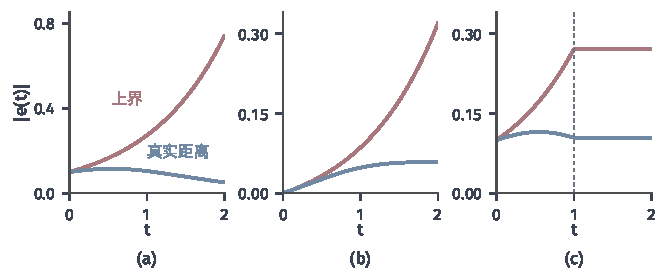
\includegraphics[width=112mm]{figures/06-differential-equations/01-ordinary-differential-equations/matplotlib/odesens-gronwall-roles/figure.pdf}
  \caption{Gronwall上界的三个成分。方程基于$\dot{x}=\sin x$，$x(0)=1$，蓝线是由数值积分得到的真实距离，红线是式~\eqref{eq:odesens-basic-estimate}的上界。(a)只有初值差$0.1$，上界$0.1\mathrm{e}^{t}$。(b)只有持续外力$r\equiv0.05$，上界$0.05(\mathrm{e}^{t}-1)$。(c)右端乘以$\beta(t)$，$\beta$在$[0,1)$上为$1$、此后为$0$，上界在$t=1$（虚线）后不再增长。}
  \label{fig:odesens-gronwall-roles}
\end{BookInlineFigure}

上界并非总是宽松的。取$\dot{x}=x$和$\dot{y}=y+0.05$，初值差$0.1$，误差方程$\dot{e}=e+0.05$可以直接解出，
\[
 e(t)=0.1\,\mathrm{e}^{t}+0.05\,(\mathrm{e}^{t}-1).
\]
这恰好是式~\eqref{eq:odesens-constant-estimate}取$L=1$、$\delta=0.05$的右端，在$t=1$时等于$0.2718+0.0859=0.3577$。可见不增加其他结构时，这个上界不能再改进。

\paragraph{去掉Lipschitz条件会怎样}
定理的结论蕴含唯一性：取$\bm{r}=\bm{0}$、$\bm{y}_0=\bm{x}_0$，上界为零。方程$\dot{x}=2\sqrt{\lvert x\rvert}$从$x(0)=0$出发有一族解，对任意$c\geq0$，
\[
 x_c(t)=\begin{cases}0,&t\leq c,\\(t-c)^2,&t>c,\end{cases}
\]
都满足方程，见图~\ref{fig:odesens-nonlipschitz-split}。比较$x_0(t)=t^2$与零解，差商是
\[
 \frac{\lvert f(t^2)-f(0)\rvert}{t^2}=\frac{2}{t},
\]
它在$t=0$附近不可积。放大系数的积分发散，式~\eqref{eq:odesens-basic-estimate}无从写起，这就是Lipschitz条件失效的具体样子。

\begin{BookInlineFigure}
  \centering
  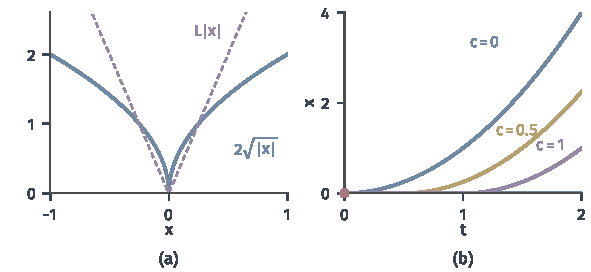
\includegraphics[width=100mm]{figures/06-differential-equations/01-ordinary-differential-equations/matplotlib/odesens-nonlipschitz-split/figure.pdf}
  \caption{没有Lipschitz条件时比较定理失效。(a)右端$2\sqrt{\lvert x\rvert}$在$x=0$处切线竖直，任何过原点的直线$L\lvert x\rvert$（紫色虚线）都压不住它。(b)同一红色初值$x(0)=0$出发的解$x_c$，$c=0,0.5,1$，蓝色水平线是零解。初值差为零，解的差却不为零。}
  \label{fig:odesens-nonlipschitz-split}
\end{BookInlineFigure}
